\documentclass[a4paper]{article}
\usepackage[margin=3cm]{geometry}
\usepackage{graphicx}

\usepackage{hyperref}
\hypersetup{
	colorlinks=true,
	linkcolor=blue,
	filecolor=magenta,
	urlcolor=cyan,
	hyperindex=true,
	linktocpage=true,%makes the page number be the link in the index
}

\renewcommand{\arraystretch}{1.2}

\title{Mind uploading through machine learning approximation of single neurons}

\author{Chaya2766}

\begin{document}
	\sffamily
	\hyphenchar\font=-1
	\sloppy
	
	\maketitle
	
	\vfill
	
	\begin{abstract}
		Calculations of the computational resources required to create and run a human brain emulation based on the paper "Single cortical neurons as deep artificial neural networks" by David Beniaguev, Idan Segev \& Michael London.
		
		\medskip
		
		I make some additional suggestions for how the data necessary might be acquired in the first place, as well as guesses as to what important considerations there might be to such a process.
	\end{abstract}
	
	%\noindent \rule{\linewidth}{1pt}
	\vfill
	
	\tableofcontents
	
	\pagebreak
	
	\section{Mimic neurons}
	
	I need to introduce a new piece of vocabulary to make the explanations less convoluted: a \textbf{mimic neuron} will be used throughout this document to refer to \underline{a neural network trained to mimic the spiking behaviour of a natural human neuron}.
	
	\medskip
	
	The paper "Single cortical neurons as deep artificial neural networks" by David Beniaguev, Idan Segev \& Michael London describes how the previously used models of biological neurons could be replaced with less computationally expensive artificial neural networks. They managed to train artificial neural networks to mimic the activity of a conventionally modeled biological neuron with more than 99\% accuracy.
	
	\medskip
	
	The artificial neural networks in the paper start with neurons which each recieve 100 streams of inputs representing input to the neuron's synapses. From this a deep neural network follows, arranged in layers, until two artificial neurons at the end, of which one returns voltage within the neuron and the other the spikes, in timesteps of 1 millisecond.
	
	\medskip
	
	\begin{minipage}{0.5\linewidth}
		I am not entirely sure of my interpretation, but as I understand it, the structure of such a mimic neuron could be visualized like this, where the example illustration on the right would show a mimic neuron with 8 input streams each having 4 milliseconds of history, and a main body with 3 layers of 4 neurons each.
	\end{minipage}
	\begin{minipage}{0.5\linewidth}
		\begin{center}
			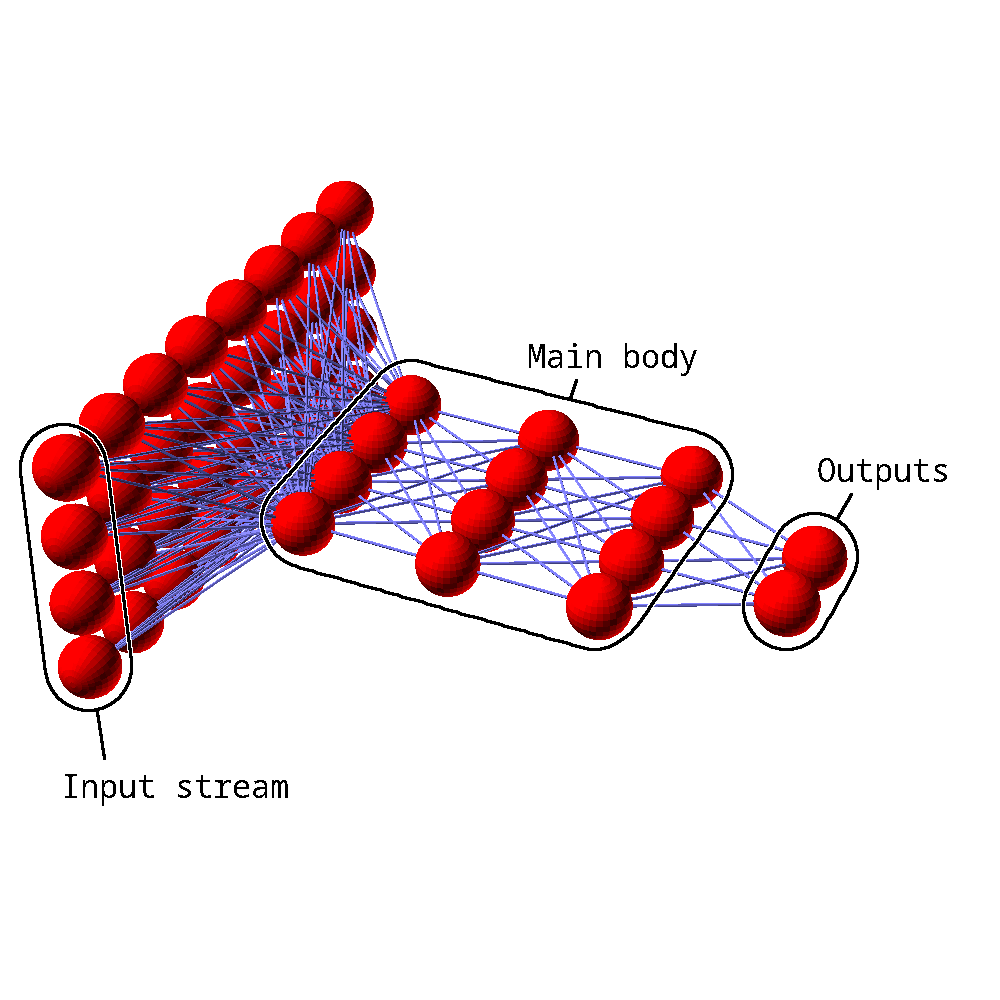
\includegraphics[width=0.8\linewidth]{mimic_neuron_example.png}
		\end{center}
	\end{minipage}
	
	
	In the study, a network with 5 layers of 128 neurons, which takes into account 205 miliseconds of input (among a number of other networks) was found to accurately model an L5PC biological neuron with AMPA \& NMDA synapses, which from not being an expert to know exactly what it means I just treat as "a lot of internal complexity".
	
	\medskip
	
	Just for visualization sake, such a mimic neuron with 100 input streams, 205 miliseconds of history in each input stream, and a main body consisting of 7 layers each having 128 neurons, would look like this:
	%TODO wrong number of layers
	%I said 7 layers but that's a mistake, I should have said 5 layers like the network from the study that I'm talking about
	%I also rendered it with 7 layers so both that sentence and the render are wrong
	%this took 1.5 hours to render, but no matter, I sink more time than that into the calculator, the render at least makes itself alone while I'm away
	%if you ever calculated for hours only to realize that somewhere along the way you accidentally started using the diameter of an object as its radius, you know
	
	\begin{center}
		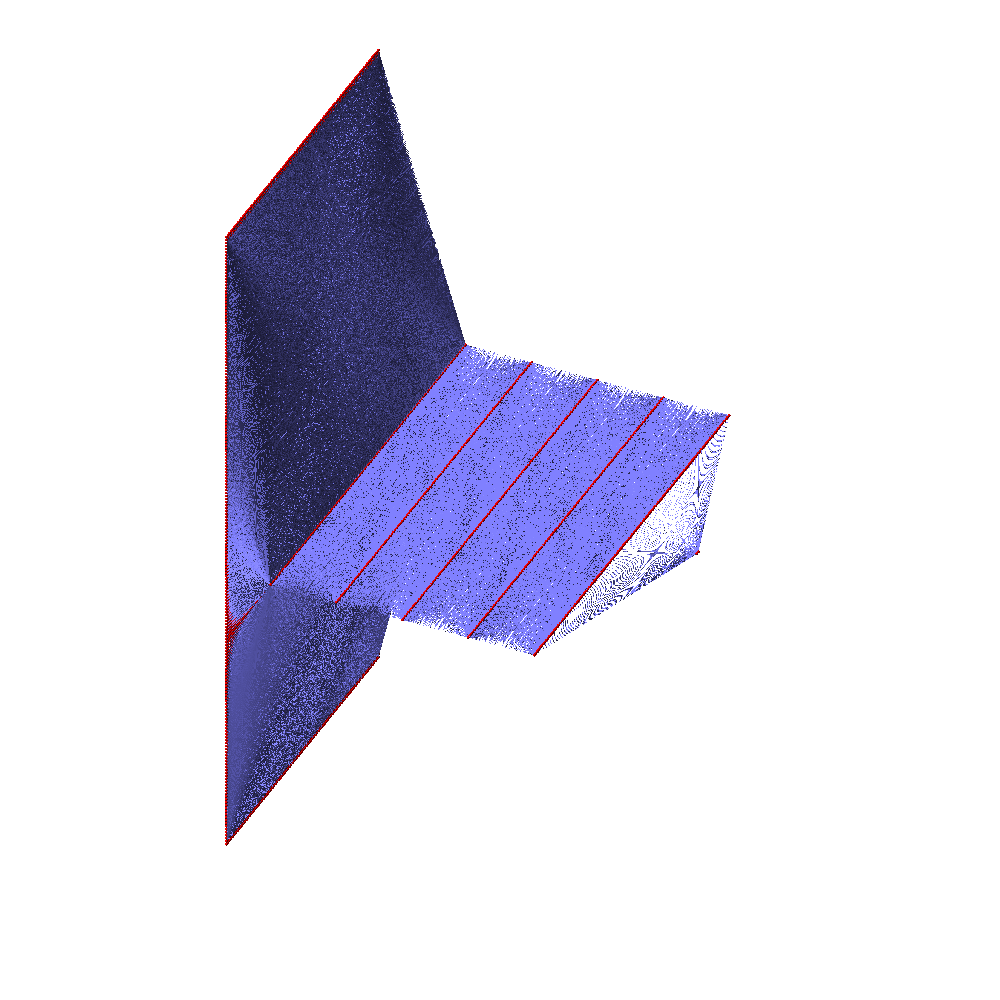
\includegraphics[width=0.5\linewidth]{mimic_neuron_real_100.png}
	\end{center}
	
	I will include the code I used to make these visualizations at the end of the document.
	
	\pagebreak
	
	Given the structure that I assumed the mimic neuron would have, a simple formula can be made for the number of parameters in the mimic neuron:
	
	$$N_w = (S \times H \times W) + ( W^2 \times (D-1)) + 2W$$
	
	Where:
	
	\smallskip
	
	\begin{itemize}
		\item $N_w$ is the total Number of Weights in the network
		
		\item $S$ is the number of input Streams which the input neurons receive
		
		\item $H$ is the history, ie. the length of each input stream
		
		\item $W$ is the width of the network, ie. number of neurons in one layer
		
		\item $D$ is the depth of the network, ie. number of layers in the main body
	\end{itemize}
	
	\medskip
	
	$(S \times H \times W)$ is the number of connections between all the input streams and all the neurons in the first layer of the main body, $( W^2 \times (D-1))$ is the total number of connections across all the layers in the main body, and $2W$ is the number of connections between the last layer of the main body and the two output neurons.
	
	\medskip
	
	The study presented several networks (their depth, width \& history) which reached past the 99\% accuracy threshold. I am setting the number of input streams to 7000, as that appears to be the number of synapses that the average human neuron has (\href{https://bionumbers.hms.harvard.edu/bionumber.aspx?id=112055}{source}).
	
	\medskip
	
	Given that assumption, the number of parameters in these networks would be:
	
	\begin{center}
		\begin{tabular}{c | c | c | c | c | r}
			number & Depth & Width & history & accuracy & num. of weights \\ \hline
			1 & 5 & 128 & 205ms & 99.13\% & 183 778 560 \\ \hline
			2 & 7 & 128 & 153ms & 99.11\% & 137 186 560 \\ \hline
			3 & 8 & 256 & 97ms & 99.14\% & 174 217 728 \\ \hline
			4 & 8 & 256 & 161ms & 99.24\% & 288 905 728 \\
		\end{tabular}
	\end{center}
	
	There appears to be a pattern of more computationally expensive networks being more accurate, though the jump from 99.11\% to 99.24\% accuracy brought more than a factor of 2 increase in computational cost, so the benefits are diminishing, at least based on this sample.
	
	\medskip
	
	The obvious choice is \underline{network 2} if wanting to minimize computational costs.
	
	\bigskip
	
	Each of the 137 186 560 parameters in the mimic neuron correspond to a multiply-and-accumulate (MAC) operation which has to be performed to fully calculate its response. The simulation is quantized in 1 millisecond intervals, which means that the neuron would require \textbf{137 186 560 000 MAC/s} to be simulated at realtime speed. Some hardware can efficiently perform MAC operations, but for more standard computing it would otherwise be two floating point operations, a multiplication and an addition, so it translates to \textbf{274 373 120 000 FLOPS}. Alternatively for a more down to physics metric, assuming that a 16-bit MAC operation requires about 2000 bit flips in total, the required bit flip rate would be \textbf{274~373~120~000~000~bits/s}
	
	\medskip
	
	Assuming 16-bit weights, the mimic neuron would require \textbf{274.37312 MB} to store. Here's a summary:
	
	\medskip
	
	\begin{center}
		\begin{tabular}{| c | c |}
			\hline
			\multicolumn{2}{|c|}{Mimic neuron} \\\hline
			accuracy to real human neuron & 99.11\% \\\hline
			number of parameters: & 137 186 560 \\\hline
			computation requirement: & 137 186 560 000 MAC/s \\
			& 274 373 120 000 FLOPS \\
			& 274 373 120 000 000 bits/s \\\hline
			size on disk or in memory: & 274.37312 MB \\\hline
		\end{tabular}
	\end{center}
	
	\pagebreak
	
	\section{Human brain on mimic neurons}
	
	There are about 86 billion neurons in the human brain. A simple multiplication of the mimic neuron's requirements by that many neurons would yield these numbers:
	
	\begin{center}
		\begin{tabular}{| c | c |}
			\hline
			\multicolumn{2}{|c|}{Human brain emulation via mimic neurons} \\\hline
			number of parameters: & 11 798 044 160 000 000 000 \\\hline
			computation requirement: & 11 798 044 160 000 000 000 000 MAC/s \\
			& 23 596 088 320 000 000 000 000 FLOPS \\
			& 23 596 088 320 000 000 000 000 000 bits/s \\\hline
			size on disk or in memory: & 23.59608832 EB \\\hline
		\end{tabular}
	\end{center}
	
	Given those numbers, I've gone ahead and calculated the amount of hardware and power required to run the emulation based on a number of devices whose parameters I was able to find:
	
	\begin{itemize}
		\item AMD Alveo V70 AI accelerator card : 2.693teraFLOPS per watt , 202teraFLOPS per device
		
		\item Halio-8 AI Accelerator : 10.4TOPS per watt , 26TOPS per device \newline (what kind of operation though? I'll just assume FLOPS for now)
		
		\item Epiphany V 1024-core RISC processor : 75gigaFLOPS per watt , ??? FLOPS per device
		
		\item JUPITER supercomputer, top of Green500 list for june 2024 : \newline 72.73gigaFLOPS per watt , 4.5petaFLOPS per device
		
		\item Frontier supercomputer, top of TOP500 list for jume 2024 : \newline 52.93gigaFLOPS per watt , 1.206exaFLOPS per device
		
		\item PTC, The photonic tensor core described in a paper "Photonic Tensor Cores for Machine Learning" by Mario Miscuglio \& Volker J. Sorger : 16 petaFLOPS per device, 8 petaFLOPS per watt\newline
		note: it uses 4-bit operations rather than my assumed 16-bit
		
		%\item Taichi photonic chiplet : \newline 160 tera-operations (I assume multiply-accumulates) per joule , ??? per second
		
		\item Nvidia H100 (\href{https://cdn.prod.website-files.com/6473d8d02a3cf26273f27856/64dfa0a0787511212d0575e0_h100-datasheet-2430615.pdf}{link to datasheet}) - 4.32286 teraFLOPS per watt, 1513 teraFLOPS (FP16) per device
		
		%\item Tesla Dojo D1 chip (\href{https://en.wikipedia.org/wiki/Tesla_Dojo#D1_chip}{wikipedia}) - 9 petaFLOPS (BF16) per device
		
		\item \href{https://lightmatter.co/blog/a-new-kind-of-computer/}{Lightmatter experimental card}: 65.5TeraFLOPS at 78W $\approx$ 839.7436GigaFLOPS per watt
		
		\item Orion's Arm \href{https://www.orionsarm.com/eg-article/48507b746e356}{Ultimate Chip} (fictional): 5.09911 E21 bits/s per device at 100W $\approx$ 1.96112655~E-20~J/bit
		
		%\item Landauer core (fictional) - perform computation exactly at landauer's limit
	\end{itemize}
	
	\medskip
	
	%I'll place a V after those which I recalculated
	
	\begin{center}
		\begin{tabular}{c | r | r}
			device & wattage & amount needed \\ \hline
			Alveo V70 & 8.768GW & 116 812 318.4 \\ \hline%V
			Halio-8 & 2.269GW & 907 541 858.5 \\ \hline%V
			Epiphany V & 314.6GW & ? \\ \hline%V
			JUPITER & 324.4GW & 5 243 575.2 \\ \hline%V
			Frontier & 445.8GW & 19 565.6 \\ \hline%V
			PTC & \textbf{2.95MW} & 1 474 755.5 \\ \hline%V
			%Taichi & 180.566MW & ? \\ \hline
			Nvidia H100 & 5.458GW & 271 852 \\ \hline
			Lightmatter experimental card & 28.1GW & 360 245 623.2 \\ \hline
			Ultimate Chip (fictional) & 462.75kW & 4627.5 \\ \hline%V
			%Landauer's limit (room temp 300K) & 164 727.23W & - \\ \hline
			%Landauer's limit (cosmic background 2.73K) & 1499.02W & -
		\end{tabular}
	\end{center}
	
	\pagebreak
	
	Problems with this approach:
	
	\medskip
	
	\textbf{1. static structure}: A healthy human brain is constantly rewiring itself, but the mimic neurons have no ability to grow new connections, and in a brain made from them they will never die, nor will new ones be born without intervention.
	
	\pagebreak
	
	\section{A suggestion on gathering the data}
	
	The method I propose for gathering data is to infiltrate the brain with roughly 86 billion probes made from nested carbon (conductive) and boron nitride (insulating) nanotubes, which are to act as data cables directly transmitting the neuron potential to measurement devices. The probes would be tipped with microscopic machines capable of swimming through the brain and navigating around its structures using power supplied to them through the probes, and at the end of their journey hooking directly into the neuron membrane, thereby gaining access to the membrane potential.
	
	\medskip
	
	In the case that no scanning technology exists that can produce sufficiently high quality scans to build the needed map of connections from, the probe tips could also act as mapping devices while they make their journey. Since neurons modify their connections during their life, having the probe tips act as mapping devices even after they are embedded into the neurons would also provide a relatively convenient way of keeping track of these changes.
	
	\medskip
	
	[illustration here]
	
	\medskip
	
	Here are a number of considerations that I acknowledge to various degrees:
	
	\begin{itemize}
		\item \textbf{size:} by using nested nanotubes the probes can be made thin enough that the volume of material added to the brain is not a concern (see calculations on next page)
		
		\item the computation required for navigation through the brain tissue can be handled by external computers, as such is not an issue
		
		\item \textbf{cost:} producing the cables is likely to be extremely costly, as it requires not only growing pristene nanotubes of carbon or boron nitride which are multiple centimetres long (which is known to be possible and had already been demonstrated in the modern day) but also assembling them together into these cables - it is also not clear how one would assemble multiple independent nanotubes into one cable. The surgery itself would also require massive amounts of computing power to actively guide each of the 86 billion probes on their journey through the brain.
		
		\item \textbf{operation time:} implanting 86 billion nanoscopically thin probes into a brain is likely to be an extremely time consuming process, but at the lower bound, the probes likely can't be implanted any faster than a microbe could swim the equivalent distance, which merely rivals modern brain surgeries in time duration.
		
		\item \textbf{safety:} It is difficult to know ahead of time if neurons will not react negatively to having a probe stuck in their membrane, but it could likely be tested ahead of time on a small number of neurons which are not too important to the patient. There also exists the possibility that something could pull on the probe (movement of the implant within the body due to external forces?), but the probe tips could likely be designed to maintain a weak enough interface with the neuron that in such a case they harmlessly detach from the neuron.
	\end{itemize}
	
\end{document}